% appendix/rcuhist/RCUinLinux.tex
% SPDX-License-Identifier: CC-BY-SA-3.0

\chapter{Read-Copy Update in Linux}
\label{app:rcuhist:Read-Copy Update in Linux}

이 챕터에서는 2008년 중반 이후부터의 리눅스 커널에서의 RCU 의 역사를
설명합니다.
그 전의 RCU 의 역사에 대해서는 다른
곳~\cite{PaulEdwardMcKenneyPhD,PaulEMcKenney2008RCUOSR} 을 찾아 보시기
바랍니다.
Section~\ref{sec:app:rcuhist:RCU Usage Within Linux}
은 리눅스에서의 RCU 사용의 증가를 개괄적으로 알아보고
Section~\ref{sec:app:rcuhist:RCU Evolution}
는 최근의 RCU 의 진화에 대한 자세한 설명을 제공합니다.
\iffalse

This chapter gives a history of RCU in the Linux kernel from mid-2008
onwards.
Earlier history of RCU may be found
elsewhere~\cite{PaulEdwardMcKenneyPhD,PaulEMcKenney2008RCUOSR}.
Section~\ref{sec:app:rcuhist:RCU Usage Within Linux}
gives an overview of the growth of RCU usage in Linux and
Section~\ref{sec:app:rcuhist:RCU Evolution}
presents a detailed view of recent RCU evolution.
\fi

\section{RCU Usage Within Linux}
\label{sec:app:rcuhist:RCU Usage Within Linux}

\begin{figure}[bp]
\centering
\resizebox{3in}{!}{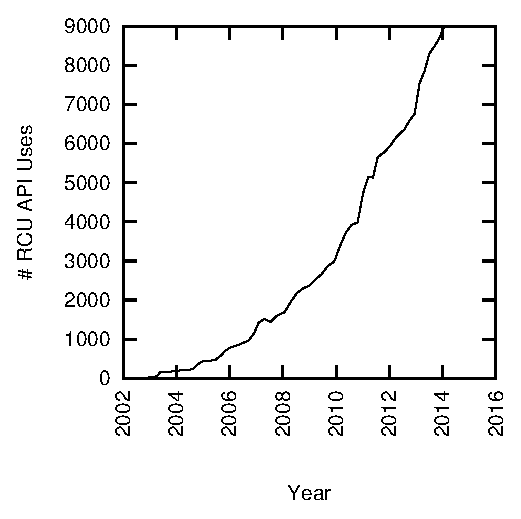
\includegraphics{appendix/rcuhist/linux-RCU}}
\caption{RCU API Usage in the Linux Kernel}
\label{fig:app:rcuhist:RCU API Usage in the Linux Kernel}
\end{figure}

\begin{figure}[bp]
\centering
\resizebox{3in}{!}{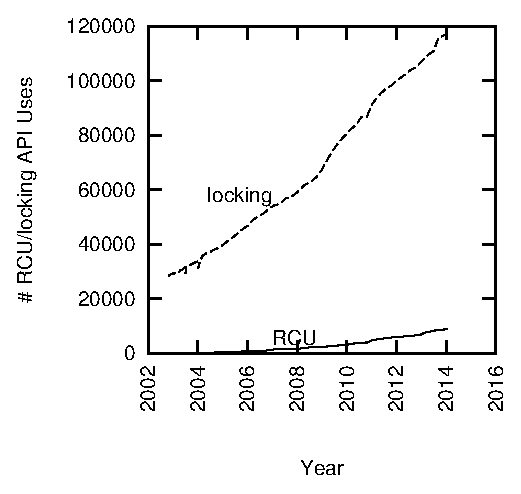
\includegraphics{appendix/rcuhist/linux-RCUlock}}
\caption{RCU API Usage in the Linux Kernel vs. Locking}
\label{fig:app:rcuhist:RCU API Usage in the Linux Kernel vs. Locking}
\end{figure}

\begin{figure}[tbp]
\centering
\resizebox{3in}{!}{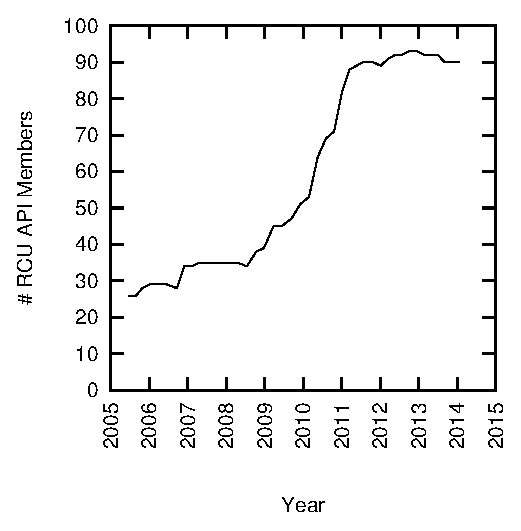
\includegraphics{appendix/rcuhist/rcuAPI}}
\caption{RCU API Growth Over Time}
\label{fig:app:rcuhist:RCU API Growth Over Time}
\end{figure}

리눅스 커널의 RCU 사용은
Figure~\ref{fig:app:rcuhist:RCU API Usage in the Linux Kernel}~\cite{PaulEMcKenneyRCUusagePage}
를 통해 볼 수 있듯이 시간에 따라 증가되었습니다.
RCU 는 코드 내에 존재하는 다른 동기화 메커니즘 (예를 들면, 네트워킹 프로토콜
스택의 \co{brlock}~\cite{Molnar00a,Torvalds2.5.69,Torvalds2.5.70}) 들을
대체했으며, 새로운 기능을 구현하는 코드 (예를 들면,
SELinux~\cite{JamesMorris04b} 에서의 audit 시스템) 와 함께 나타나기도 했습니다.
하지만, RCU 는
Figure~\ref{fig:app:rcuhist:RCU API Usage in the Linux Kernel vs. Locking} 에
보여지듯이 락킹에 비해서 틈새에만 사용되는 기술로 남아있습니다.
락킹이 커널 해커의 동시성 도구상자의 망치라면, RCU 는 아마도
스크류드라이버입니다.
만약 그렇다면,
Figure~\ref{fig:app:rcuhist:RCU API Growth Over Time} 를 통해 볼 수 있듯 매우
급격히 성장하는 스크류드라이버입니다.
\iffalse

The Linux kernel's usage of RCU has increased over the years,
as can be seen from
Figure~\ref{fig:app:rcuhist:RCU API Usage in the Linux Kernel}~\cite{PaulEMcKenneyRCUusagePage}.
RCU has replaced other synchronization mechanisms
in existing code
(for example, \co{brlock} in the networking protocol
stacks~\cite{Molnar00a,Torvalds2.5.69,Torvalds2.5.70}),
and it has also been introduced with code implementing
new functionality
(for example, the audit system within SELinux~\cite{JamesMorris04b}).
However, RCU remains a niche technology compared to locking,
as shown in
Figure~\ref{fig:app:rcuhist:RCU API Usage in the Linux Kernel vs. Locking}.
If locking is the hammer in the kernel hacker's concurrency toolbox,
perhaps RCU is the screwdriver.
If so, it is an rapidly evolving screwdriver, as can be seen in
Figure~\ref{fig:app:rcuhist:RCU API Growth Over Time}.
\fi

\section{RCU Evolution}
\label{sec:app:rcuhist:RCU Evolution}

이 섹션은 2008년 중반 이후 계속 진행중인 RCU 에 대한 경험을 제공합니다.
\iffalse

This section presents ongoing experience with RCU since mid-2008.
\fi

\subsection{2.6.27 Linux Kernel}

This release added the
\co{call_rcu_sched()},
\co{rcu_barrier_sched()}, and
\co{rcu_barrier_bh()} RCU API members.

\subsection{2.6.28 Linux Kernel}

RCU API 의 크기를 실제로 줄이는데에 관련된 변경사항으로
\co{list_for_each_rcu()} 기능의 제거가 있었습니다.
이 기능은 \co{list_head} 구조체를 구성하는 포인터쌍을 따라가기보다는 (헷갈릴 수
있지만, 리스트 헤더뿐 아니라 리스트 원소로 동작하는) 구조체들을 따라가는 장점을
가진 \co{list_for_each_entry_rcu()} 로 대체되었습니다.
이 변경은 2.6.28 리눅스 커널에 받아들여졌습니다.

안타깝게도, 2.6.28 리눅스 커널은 또한 \co{rcu_read_lock_sched()} 와
\co{rcu_read_unlock_sched()} RCU API 멤버들을 추가했습니다.
이 API 들은 가독성을 올리기 위해 추가되었습니다.
과거에는, \co{synchronize_sched()} 에 연관된 RCU read-side 크리티컬 섹션들을
표시하기 위해 인터럽트나 preemption 을 불능화 시키는데 사용되는 기능들을
사용했습니다.
하지만, 이는 개발자들이 preemption 이나 인터럽트를 불능화 시킬 필요가
없어졌지만 RCU 보호를 위한 필요를 알지 못할 때에 버그가 생기도록 이끌었습니다.
\co{rcu_read_lock_sched()} 의 사용은 그런 버그를 예방하는데 도움이 될 것입니다.
\iffalse

One welcome change involved an actual reduction in the size of RCU's
API with the removal of the \co{list_for_each_rcu()} primitive.
This primitive is superseded by \co{list_for_each_entry_rcu()},
which has the advantage of iterating over structures rather than
iterating over the pointer pairs making up a \co{list_head}
structure (which, confusingly, acts as a list element as well
as a list header).
This change was accepted into the 2.6.28 Linux kernel.

Unfortunately, the 2.6.28 Linux kernel also added
\co{rcu_read_lock_sched()} and
\co{rcu_read_unlock_sched()} RCU API members.
These APIs were added to promote readability.
In the past, primitives to disable interrupts or preemption were used
to mark the RCU read-side critical sections corresponding to
\co{synchronize_sched()}.
However, this practice led to bugs when developers removed the need
to disable preemption or interrupts, but failed to notice the need
for RCU protection.
Use of \co{rcu_read_lock_sched()} will help prevent such bugs in the
future.
\fi

\subsection{2.6.29 Linux Kernel}

새로운 더욱 확장성 있는 구현, ``Tree RCU'' 가 bitmap 을 combining tree 로
대체하면서 2.6.29 리눅스 커널에 받아들여졌습니다.
이 구현은 근래의 멀티프로세서들의 계속해서 증가하는 코어의 갯수에서 영감을
받아서 수백개의 CPU 환경을 위해 설계되었습니다.
현재의 구조상의 한계는 262,144 개 CPU 인데, 이는 개발자들이 (순진한 것일 수도
있지만) 한동안은 충분할 것이라 믿는 숫자입니다.
이 구현은 또한 preemptible RCU 의 개선된 dynamic-tick 인터페이스 인터페이스를
받아들였습니다.
\iffalse

A new more-scalable implementation, dubbed ``Tree RCU'', replaces
the flat bitmap with a combining tree, and was accepted into the 2.6.29
Linux kernel.
This implementation was inspired by the ever-growing core counts of
modern multiprocessors, and is designed for many hundreds of CPUs.
Its current architectural limit is 262,144 CPUs, which the developer
(perhaps na\"ively) believes to be sufficient for quite some time.
This implementation also adopts preemptible RCU's improved dynamic-tick
interface.
\fi

Mathieu Desnoyers 는 리눅스 커널의 tracing code 가 RCU 를 사용하도록 하는데
필요한 \co{rcu_read_lock_sched_notrace()} 와
\co{rcu_read_unlock_sched_notrace()} 를 추가했습니다.
이 API 들 없이는, RCU read-side 크리티컬 섹션을 추적하려는 시도는 무한 재귀
문제를 일으킵니다.
\iffalse

Mathieu Desnoyers added
\co{rcu_read_lock_sched_notrace()} and
\co{rcu_read_unlock_sched_notrace()},
which are required to permit the tracing code in the Linux kernel
to use RCU.
Without these APIs, attempts to trace RCU read-side critical sections
lead to infinite recursion.
\fi

Eric Dumazet 은 리스트 포인터에 단일 비트 마커들이 저장될 수 있도록 하는 새로운
종류의 RCU 로 보호되는 리스트를 추가했습니다.
이 종류의 리스트는 여러개의 락이 없는 알고리즘들을 가능하게 하는데, Maged
Michael 에 의해 보고된 것~\cite{MagedMichael04a} 등을 포함합니다.
Eric 의 작업은 \co{hlist_nulls_add_head_rcu()}, \co{hlist_nulls_del_rcu()},
\co{hlist_nulls_del_init_rcu()}, 그리고 \co{hlist_nulls_for_each_entry_rcu()}
를 추가합니다.
이는 또한 \co{hlist_nulls_node} 라는 이름의 새로운 구조체를 추가합니다.

또한, 이건 엄격히 말해서 리눅스 커널의 부분은 아니긴 하지만, 동시에 Mathieu
Desnoyers 는 그의 유저스페이스 RCU 구현~\cite{MathieuDesnoyers2009URCU} 을
발표했습니다.
이는 real-time user-level RCU 구현을 향한 중요한 첫걸음입니다.
\iffalse

Eric Dumazet added a new type of RCU-protected list that allows single-bit
markers to be stored in the list pointers.
This type of list enables a number of lockless algorithms, including
some reported on by Maged Michael~\cite{MagedMichael04a}.
Eric's work adds the \co{hlist_nulls_add_head_rcu()},
\co{hlist_nulls_del_rcu()}, \co{hlist_nulls_del_init_rcu()}, and
\co{hlist_nulls_for_each_entry_rcu()}.
It also adds a new structure named \co{hlist_nulls_node}.

Although it is strictly speaking not part of the Linux kernel, 
at about this same time, Mathieu Desnoyers announced his user-space
RCU implementation~\cite{MathieuDesnoyers2009URCU}.
This is an important first step towards a real-time user-level RCU
implementation.
\fi

\subsection{2.6.31 Linux Kernel}

Jiri Pirko 는 RCU-subscription 기능인 \co{rcu_dereference()} 를 더 높은 수준의
리스트 접근 기능에 포함시킨 \co{list_entry_rcu} 와 \co{list_first_entry_rcu()}
기능을 추가했는데, 이 기능들은 일련의 버그들을 제거해줄 수 있을 겁니다.

또한, ``Tree RCU'' 구현은 ``experimental'' 상태로부터 업그레이드 되었습니다.
\iffalse

Jiri Pirko added \co{list_entry_rcu} and \co{list_first_entry_rcu()}
primitives that encapsulate the \co{rcu_dereference()} RCU-subscription
primitive into higher-level list-access primitives, which will hopefully
eliminate a class of bugs.

In addition, the ``Tree RCU'' implementation was upgraded from
``experimental'' status.
\fi

\subsection{2.6.32 Linux Kernel}

리눅스 커널의 이 버전에서의 가장 큰 변경은 ``Classic RCU'' 구현의 제거일
것입니다.
이 구현은 ``Tree RCU'' 구현으로 대체되었습니다.

이 버전은 그 외에도 여러 변경을 가졌는데, 다음과 같은 것들이 포함됩니다:
\iffalse

Perhaps the largest change in this version of the Linux kernel
is the removal of the old ``Classic RCU'' implementation.
This implementation is superseded by the ``Tree RCU'' implementation.

This version saw a number of other changes, including:
\fi

\begin{enumerate}
\item	\co{synchronize_rcu_expedited()}, \co{synchronize_sched_expedited()},
	그리고 \co{synchronize_rcu_bh_expedited()} RCU API 멤버들의 추가.
	이 기능들은 grace period 를 신속히 처리하기 위해 측정을 한다는 점을
	제외하고는 non-expedited 버전의 것들과 동일합니다.
\item	``Tree RCU'' 구현에 preemptible-RCU 기능들을 추가함으로써 리눅스로
	돌아가는 커다란 멀티프로세서 머신에서의 real-time response 에 대한
	문제를 해결.
\item	이 새로운 ``Tree Preemptible RCU'' 구현은 기존의 preemptible RCU 구현을
	구형으로 만들어서 리눅스 커널에서 사라지게 했습니다.
\iffalse

\item	The appearance of \co{synchronize_rcu_expedited()},
	\co{synchronize_sched_expedited()}, and
	\co{synchronize_rcu_bh_expedited()} RCU API members.
	These primitives are equivalent to their non-expedited
	counterparts, except that they take measures to expedite the
	grace period.
\item	Add preemptible-RCU functionality to the ``Tree RCU''
	implementation, thus removing one obstacle to real-time
	response from large multiprocessor machines running Linux.
\item	This new ``Tree Preemptible RCU'' implementation obsoletes
	the old preemptible RCU implementation, which was removed
	from the Linux kernel.
\fi
\end{enumerate}

\subsection{2.6.33 Linux Kernel}

이 릴리즈에서의 가장 극적인 추가사항은 Tree RCU 에서의 day-one
버그~\cite{PaulEMcKenney2009HuntingHeisenbugs} 였을 겁니다.
다른 변경 사항들은 다음과 같습니다:
\iffalse

Perhaps the most dramatic addition to this release was
a day-one bug in Tree RCU~\cite{PaulEMcKenney2009HuntingHeisenbugs}.
Other changes include:
\fi

\begin{enumerate}
\item	``RCU: The Bloatwatch
	Edition''~\cite{PaulEMcKenney2009LWNBloatWatchRCU} 라고도 알려진 ``Tiny
	RCU''.
\item	\co{synchronize_srcu_expedited()} 의 형태의 expedited SRCU.
\item	앞서 이야기된 버그에 의해 촉발된 Tree RCU 동기화의 정리.
\item	Tree Preemptible RCU 의 expedited 구현의 추가 (이전의 릴리즈에서,
	``expedited'' 지원은 단순히 \co{synchronize_rcu()} 로 매핑되었는데,
	이는 의미적으로는 옳은 동작이지만 성능 관점에서는 별로 도움이 되지
	않았습니다.)
\item	스트레스 테스트를 향상시킨 네번째 수준의 Tree RCU 추가.
	이로 인해, 누군가가 16,777,216 개의 CPU 를 가진 시스템에서 리눅스를
	돌리고자 한다면, RCU 를 그런 환경에도 준비가 되었습니다!
	대략 1600 만개의 per-CPU 데이터 원소들을 스캐닝 하는 것에 대한 응답시간
	의미 \ldots
\iffalse

\item	``Tiny RCU'', also known as ``RCU: The Bloatwatch
	Edition''~\cite{PaulEMcKenney2009LWNBloatWatchRCU}.
\item	Expedited SRCU in the form of
	\co{synchronize_srcu_expedited()}.
\item	A cleanup of Tree RCU synchronization prompted by the
	afore-mentioned bug.
\item	Add expedited implementation for Tree Preemptible RCU
	(in earlier releases, ``expedited'' support had simply
	mapped to \co{synchronize_rcu()}, which is semantically
	correct if somewhat unhelpful from a performance viewpoint.)
\item	Add a fourth level to Tree RCU, which improves stress testing.
	Therefore, if someone ever wants to run Linux on a system with
	16,777,216 CPUs, RCU is ready for them!
	Give or take the response-time implications of scanning
	through 16 million per-CPU data elements \ldots
\fi
\end{enumerate}

\subsection{2.6.34 Linux Kernel}

이 릴리즈에서 가장 눈에 띄는 추가사항은 \co{rcu_dereference()} 가 올바른 락킹
조건을 체크하도록 하는 \co{CONFIG_PROVE_RCU}~\cite{PaulEMcKenney2010LockdepRCU}
였습니다.
다른 변경들은 다음과 같습니다:
\iffalse

The most visible addition for this release was \co{CONFIG_PROVE_RCU},
which allows \co{rcu_dereference()} to check for correct locking
conditions~\cite{PaulEMcKenney2010LockdepRCU}.
Other changes include:
\fi

\begin{enumerate}
\item	기존 grace period 를 강제하고 새로운 grace period 를 시작하는 사이의
	Tree RCU 의 상호작용의 간소화.
\item	Free-running 카운터들이 부호 없게 되도록 카운터들을 재작업.
	(C-컴파일러 해커들이 부호 있는 정수를 오버플로우 시킴으로써 코드를
	깨먹을 수 있는 최적화를 이야기 하면서 얼굴에 띄웠던 즐거운 표정을
	여러분은 상상하지도 못할겁니다!!!)
\item	RCU read-side 크리티컬 섹션 안에서 지나치게 많은 시간 동안 preemption
	당한 모든 태스크들을 출력하기 위한 Tree Preemptible RCU 의 stall 파악
	기능 업데이트.
\item	Tree RCU 의 CPU-stall-detection 코드의 다른 버그 수정과 개선.
	이 코드는, 예를 들어, 인터럽트가 불능화 된채 무한루프를 돌거나 하는,
	락업된 CPU 들을 체크합니다.
\item	배터리로 동작하는 멀티프로세서 시스템에서 마지막 CPU 가 idle 상태로
	빠질 때 grace period 를 가속화 시키기 위한 일부 코드를 프로토타입.
	시스템이 모든 CPU 들이 꺼질 수 있는 상태로 넘어가는데에 추가적인 몇
	밀리세컨드를 RCU 가 가져가는데에 대해서 상당히 불쾌해 했던 사람들이
	존재합니다!
\iffalse

\item	Simplifying Tree RCU's interactions between
	forcing an old grace period and starting a new one.
\item	Rework counters so that free-running counters are unsigned.
	(You simply cannot imagine the glee on the faces of certain
	C-compiler hackers while they discussed optimizations that would
	break code that naively overflowed signed integers!!!)
\item	Update Tree Preemptible RCU's stall detection to print out
	any tasks preempted for excessive time periods while in
	an RCU read-side critical section.
\item	Other bug fixes and improvements to Tree RCU's CPU-stall-detection
	code.
	This code checks for CPUs being locked up, for example,
	in infinite loops with interrupts disabled.
\item	Prototype some code to accelerate grace periods when the
	last CPU goes idle in battery-powered multiprocessor
	systems.
	There were people who were quite unhappy about RCU taking
	a few extra milliseconds to get the system in a state
	where all CPUs could be powered down!
\fi
\end{enumerate}

\subsection{2.6.35 Linux Kernel}

이 릴리즈는 여러개의 버그 수정과 코드 정리를 추가합니다.
여기서의 주요 변경 사항은 Mathieu Desnoyers 의 RCU 콜백의 오용을 위한 검사로,
예를 들면 하나의 grace period 안에서 \co{rcu_head} 구조체를 \co{call_rcu()} 에
두번 보내거나 하는 경우입니다.
\iffalse

This release includes a number of bug fixes and cleanups.
The major change is the first installment of Mathieu Desnoyers's
patch to check for misuse of RCU callbacks, for example, passing
a \co{rcu_head} structure to \co{call_rcu()} a second time within
a single grace period.
\fi

\subsection{2.6.36 Linux Kernel}

Mathieu Desnoyers 의 디버그 목적의 작업물의 핵심은 2.6.36 에 나타났는데, 일부
코드 정리 작업은 다른 maintainer 트리들에 나오는 커밋들과의 종속성 때문에
2.6.37 로 미뤄졌습니다.
Arnd Bergmann 의 sparse RCU 검사의 한 핵심적 부분이 2.6.36 에 나타났는데,
나머지는 역시 다른 maintainer 트리에 나오는 커밋과의 종속성 때문에 2.6.37 로
미뤄졌습니다.
마지막으로, Eric Dumazet 으로부터의 패치는 \co{rcu_dereference_bh()} 의 에러
검사에서의 에러를 고쳤습니다.
\iffalse

The core of Mathieu Desnoyers's debugobjects work appeared in 2.6.36,
with some cleanups deferred to 2.6.37 due to dependencies on commits
flowing up other maintainer trees.
A key piece of Arnd Bergmann's sparse RCU checking appeared in 2.6.36,
with the remainder deferred to 2.6.37, again due to dependencies on
commits flowing up other maintainer trees.
Finally, a patch from Eric Dumazet fixed an error in
\co{rcu_dereference_bh()}'s error checking.
\fi

\subsection{2.6.37 Linux Kernel}

Mathieu Desnoyers 의 디버그 목적 작업의 마지막 정리 작업이 2.6.37 에 Arnd
Bergmann 의 sparse 기반 검사 작업과 함께 나타났습니다.
Lai Jiangshan 은 rcutorture 에 preemption 에 의한 문제 상황을 추가했고 Tree RCU
의 per-CPU 데이터 처리를 일부 간단화 시켰습니다.
Tetsuo Handa 는 RCU lockdep 으로 나온 문제 하나를 고쳤고, Christian Dietrich 는
불필요하게 반복된 \co{#ifdef} 를 제거했으며, Dongdong Deng 은 일부 Tree RCU
제어 데이터로의 락 없는 액세스를 가능하게 하도록 \co{ACCESS_ONCE()} 를
추가했습니다.

Paul 의 preemptible Tiny RCU 의 구현 또한 RCU CPU stall-warning 코드, docbook
수정, 중복 코드의 합체, Tree RCU 속도향상, RCU callback flow 에의 queuing 모델
지원에 대한 tracing 추가, 그리고 몇가지 기타 수정과 정리 작업과 함께 2.6.37
에서 나타났습니다.
\iffalse

The final cleanups from Mathieu Desnoyers's debugobjects work appeared
in 2.6.37, as did the remainder of Arnd Bergmann's sparse-based checking work.
Lai Jiangshan added some preemption nastiness to rcutorture and
made some simplifications to Tree RCU's handling of per-CPU data.
Tetsuo Handa fixed an RCU lockdep splat, Christian Dietrich removed
a redundant \co{#ifdef}, and Dongdong Deng added an
\co{ACCESS_ONCE()} that help call out lockless accesses to some
Tree RCU control data.

Paul's implementation of preemptible Tiny RCU also appeared in
2.6.37, as did a number of enhancements to the RCU CPU stall-warning
code, docbook fixes, coalescing of duplicate code, Tree RCU speedups,
added tracing to support queuing models on RCU callback flow,
and several miscellaneous fixes and cleanups.
\fi

\subsection{2.6.38 Linux Kernel}

Lai Jiangshan 은 \co{synchronize_sched_expedited()} 를 \co{kernel/sched.c} 에서
그것이 유래한 \co{kernel/rcutree.c} 와 \co{kernel/rcu_tiny.c} 로 옮겼습니다.
그는 또한 \co{orphan_cbs_list} 를 제거함으로써 CPU-hotplug 오퍼레이션 동안의
RCU-callback 처리를 단순화 해서, offline 이 되는 CPU 에 의해 고아가 되는 RCU
콜백들이 곧바로 해당 offline 화 시키는 동작을 함께 돕는 CPU 들에 의해 곧바로
처리될 수 있도록 했습니다.
Tejun Heo 는 \co{synchronize_sched_expedited()} 의 batching 기능을 개선했는데,
이는 결국 많은 동시적 \co{synchronize_sched_expedited} 오퍼레이션들을 갖는
워크로드들의 성능과 확장성을 개선했습니다.
Fre\'ed\'eric Weisbecker 는 RCU 를 idle 상태일 때 더욱 전력에 효율적이도록
만들어주는 RCU 핵심 코드상의 일부 변경을 제공했습니다.
Mariusz Kozlowski 는 \co{__list_for_each_rcu()} 상의 문법상 에러를 고쳐졌고, 곧
사라졌습니다.
(하지만 이 고쳐진 버전은 필요한 경우를 위해 git tree 상에 존재합니다.)
Nick Piggin 은 RCU 로 보호되는 bit-locked doubly-linked list 들을 위해
\co{hlist_bl_set_first_rcu()},
\co{hlist_bl_first_rcu()},
\co{hlist_bl_del_init_rcu()},
\co{hlist_bl_del_rcu()},
\co{hlist_bl_add_head_rcu()}, 그리고
\co{hlist_bl_for_each_entry_rcu()} 기능을 추가했습니다.
Christoph Lameter 는 변수가 곧바로 접근되는 경우에 사용되기 위한
\co{__get_cpu_var()} 의 최적화된 변종인 \co{__this_cpu_read()} 를 구현했습니다.
\iffalse

Lai Jiangshan moved \co{synchronize_sched_expedited()} out of
\co{kernel/sched.c} and into \co{kernel/rcutree.c} and
\co{kernel/rcu_tiny.c} where it belongs.
He also simplified RCU-callback handling during CPU-hotplug operations
by eliminating the \co{orphan_cbs_list}, so that RCU callbacks
orphaned by a CPU that is going offline are immediately adopted by
the CPU that is orchestrating the offlining sequence.
Tejun Heo improved \co{synchronize_sched_expedited()}'s batching
capabilities, which in turn improves performance and scalability
for workloads with many concurrent \co{synchronize_sched_expedited}
operations.
Fr\'ed\'eric Weisbecker provided a couple of subtle changes to the
RCU core code that make RCU more power-efficient when idle.
Mariusz Kozlowski fixed an embarrassing syntax error in
\co{__list_for_each_rcu()}, which was then removed.
(But the fixed version is there in the git tree should it be needed.)
Nick Piggin added the \co{hlist_bl_set_first_rcu()},
\co{hlist_bl_first_rcu()},
\co{hlist_bl_del_init_rcu()},
\co{hlist_bl_del_rcu()},
\co{hlist_bl_add_head_rcu()}, and
\co{hlist_bl_for_each_entry_rcu()} primitives for RCU-protected use
of bit-locked doubly-linked lists.
Christoph Lameter implemented \co{__this_cpu_read()}, which is an
optimized variant of
\co{__get_cpu_var()} for use in cases where the variable is accessed directly.
\fi

또한, \co{TINY_RCU} 는 priority boosting 을 얻었고,
\co{synchronize_srcu_expedited()} 의 race condition 이 고쳐졌고,
\co{synchronized_srcu_expedited()} 가 동시적인 읽기 쓰레드들이 존재할 때에
expedited 본성을 얻을 수 있도록 수정되었으며, grace-period 시작/종료 검사가
개선되었고, \co{TREE_RCU} 의 leaf-level fanout 이 lock-contention 문제들을
고치기 위해 16 으로 제한되었습니다.
이 마지막 변경은 \co{TREE_RCU} 와 \co{TREE_PREEMPT_RCU} 가 지원할 수 있는 CPU
들의 최대 갯수를 4,194,304 로 줄였는데, 이는 (다시 말하지만, 어쩌면 순진하게도)
충분할 것으로 여겨집니다.
\iffalse

In addition, \co{TINY_RCU} gained priority boosting, a race condition
in \co{synchronize_sched_expedited()} was fixed,
\co{synchronize_srcu_expedited()} was modified to retain its expedited
nature in the face of concurrent readers,
grace-period begin/end checks were improved,
and the \co{TREE_RCU} leaf-level fanout was limited to 16 in order to fix
lock-contention problems.
This last change reduces the maximum number of CPUs that \co{TREE_RCU}
and \co{TREE_PREEMPT_RCU} can support down to 4,194,304, which is
(again, perhaps na\"ively) believed to be sufficient.
\fi

\subsection{2.6.39 Linux Kernel}

Lai Jiangshan 은 task 가 RCU read-side 크리티컬 섹션 내에서 종료되는 경우에
디버깅 상태를 보존하기 위해 \co{exit_rcu()} 가 \co{rcu_read_unlock()} 대신
\co{__rcu_read_unlock()} 을 호출하도록 만들었으며, Jesper Juhl 은 rcutorture
내의 중복된 \co{sched.h} 포함을 제거했고, Amerigo Wang 은 \co{rcu_fixup_free()}
로부터 의미없는 코드들을 일부 제거했습니다.

또한, MCE 서브시스템에서의 사용을 위해 새로운 \co{rcu_access_index()} 가
만들어졌습니다.
\iffalse

Lai Jiangshan made \co{TINY_RCU}'s \co{exit_rcu()} invoke
\co{__rcu_read_unlock()}
rather than \co{rcu_read_unlock()} in case of a task exiting while
in an RCU read-side critical section in order to preserve debugging
state,
Jesper Juhl removed a duplicate include of \co{sched.h} from
rcutorture,
and
Amerigo Wang removed some dead code from \co{rcu_fixup_free()}.

In addition, a new \co{rcu_access_index()} was created for use in the
MCE subsystem.
\fi

\subsection{3.0 Linux Kernel}

많은 사람들이 2.6.40 릴리즈가 될 것이라 예상했던 것은 3.0 릴리즈가 되었습니다.
여기서 가장 중요한 RCU 기능은 Tree RCU 를 위한 priority boosting 의
추가였습니다: 계획됐던 것보다 여러면에서
중요해서~\cite{PaulEMcKenney2011RCU3.0trainwreck}, 3.0-rc7 뒤의 RCU 수정이
되었습니다.
Shaohua Li, Peter Zijlstra, Steven Rostedt 의 RCU, 스케쥴러, 그리고 thread 로
돌아가는 인터럽트들 사이의 충돌의 fallout 처리에 대한 많은 도움에 감사를 드리는
바입니다.
또한, RCU CPU stall warning 들은, 여전히 커널 부트 패러미터나 \co{sysfs} 로
조정될 수 있는 \co{rcu_cpu_stall_suppress} 모듈 패러미터로 불능화 될 수 있긴
하지만, 이제 무조건적으로 Tree RCU 안으로 컴파일 됩니다.
\iffalse

What many expected to be the 2.6.40 release became instead the 3.0 release.
The most important RCU feature was the addition of priority boosting
for Tree RCU: Important in more ways than
planned~\cite{PaulEMcKenney2011RCU3.0trainwreck}, resulting in RCU
fixes after 3.0-rc7.
Kudos to Shaohua Li, Peter Zijlstra, Steven Rostedt for much help
dealing with the fallout of the collision between RCU, the scheduler,
and threaded interrupts.
In addition, RCU CPU stall warnings are now unconditionally compiled
into Tree RCU, though they may still be disabled via the
\co{rcu_cpu_stall_suppress} module parameter, which may be controlled
from either the kernel boot parameter string or \co{sysfs}.
\fi

Mathieu Desnoyers 는 non-preemptible RCU 구현에 들어오게 되는
\co{DEBUG_OBJECTS_RCU_HEAD} 체크를 활성화 시켰습니다.
Lai Jiangshan 은 fire-and-forget \co{kfree_rcu()} 를 만들었고 (그리고 이를
커널을 통해 적용했습니다), 또한 \co{exit_rcu()} 가 task 가 RCU read-side
크리티컬 섹션 내에서 끝나는 경우에 디버깅 상태를 유지할 수 있도록 하기 위해
\co{rcu_read_unlock()} 대신 \co{__rcu_read_unlock()} 을 호출하도록
만들었습니다.
Eric Dumazet 는 더 나아가서 \co{TINY_RCU} 를 감소시켰고 Gleb Natapov 는
가상화가 guest OS 와의 문맥 전환 시에 일어나는 quiescent state 들 사이에 RCU 가
신경을 쓸 수 있도록 RCU hook 들을 추가했습니다.
Peter Zijlstra 는 RCU kthread 블록킹과 wakeup 을 streamline 시켰습니다.
\iffalse

Mathieu Desnoyers enabled \co{DEBUG_OBJECTS_RCU_HEAD} checking to
be carried out in non-preemptible RCU implementations.
Lai Jiangshan created a fire-and-forget \co{kfree_rcu()} (and applied
it throughout the kernel),
and also made \co{TREE_RCU}'s \co{exit_rcu()} invoke
\co{__rcu_read_unlock()}
rather than \co{rcu_read_unlock()} in case of a task exiting while
in an RCU read-side critical section in order to preserve debugging
state.
Eric Dumazet further shrank \co{TINY_RCU} and
Gleb Natapov added RCU hooks to allow virtualization to call RCU's
attention to quiescent states that occur when switching context to
and from a guest OS.
Peter Zijlstra streamlined RCU kthread blocking and wakeup.
\fi

\subsection{3.1 Linux Kernel}

3.1 버전은 Arun Sharma, Jiri Kosina, Michal Hocko, Peter Zijlstra, 그리고 Jan
H. Sch\"{o}nherr 로부터의 마이너한 수정들과 코드 정리들을 포함한, RCU 에
있어서는 조용한 시간이었습니다.
\iffalse

The 3.1 version was a quiet time for RCU, with cleanups and minor fixes
from Arun Sharma, Jiri Kosina, Michal Hocko, Peter Zijlstra,
and Jan H. Sch\"{o}nherr.
\fi

\subsection{3.2 Linux Kernel}

3.2 리눅스 커널은 RCU 의 코드의 꼭대기부터 바닥까지의 검사 첫번째 단계에서
발견된 문제들에 대한 여러 수정사항들을 담고 있습니다.
이 검사의 결과물 가운데 하나는 코드의 irq 불능화된 구간이 preemptible RCU
read-side 크리티컬 섹션의 시작이 아니라 끝과 겹치게 되면 데드락이 일어날 수
있다는 것이었습니다.
따라서, 부분적으로 irq 불능화된 코드 구간과 겹칠 수 있는 RCU read-side 크리티컬
섹션들을 만들지 마세요:
대신에, irq 불능화된 코드 섹션을 주어진 RCU read-side 크리티컬 섹션 안에 완전히
집어넣거나 그 반대로 하거나 하세요.
\iffalse

The 3.2 Linux kernel contains a number of fixes to issues located
during the first phase of a top-to-bottom inspection of RCU's code.
One outcome of this inspection is that deadlock can occur if
an irq-disabled section of code overlaps the end but not the beginning
of a preemptible RCU read-side critical section.
Therefore, do not code RCU read-side critical sections that partially
overlap with irq-disabled code sections:
Instead, either fully enclose the irq-disable code sections within a
given RCU read-side critical section or vice versa.
\fi

이 릴리즈는 RCU 이벤트 추적 기능을 처음으로 보였습니다.
Eric Dumazet 는 RCU 의 kthread 들이 NUMA 시스템에 최적화된 방식으로 위치된
메모리를 가지게 됨을 보장하는 \co{kthread_create_on_node()} 기능을
적용했습니다.
그는 또한 \co{rcu_assign_pointer()} 가 무조건적으로 메모리 배리어를 삽입하도록
했는데, 특정 환경에서는 이 메모리 배리어가 생략되게 했던 기존의 컴파일러의
마술이 그보다 최신의 버전의 컴파일러에서는 통하지 않았기 때문입니다.
따라서, RCU 로 보호되는 포인터에 \co{NULL} 을 할당할 때에는,
\co{rcu_assign_pointer()} 보다는 \co{RCU_INIT_POIINTER()} 를 사용하세요.
\iffalse

This release saw the first RCU event-tracing capabilities.
Eric Dumazet applied the new
\co{kthread_create_on_node()} primitive to ensure that RCU's
kthreads have memory placed optimally on NUMA systems.
He also
made the \co{rcu_assign_pointer()} unconditionally insert a
memory barrier because the earlier compiler magic permitting this
barrier to be omitted under certain circumstances fails in newer
versions of the compiler.
Therefore, when assigning \co{NULL} to an RCU-protected pointer,
use \co{RCU_INIT_POINTER()} rather than \co{rcu_assign_pointer()}.
\fi

Shaohua Li 는 RCU 의 per-CPU kthread 들의 불필요한 self-wakeup 을 제거했고,
Andi Kleen 은 일부 충돌되는 변수 선언들을 정리했습니다.
Mike Galbraith 는 RCU 가 \co{RCU_BOOST_PRIO} 커널 패러미터를 무시하게 하는
버그를 잡았고, 마지막으로, 계속해서 확장되는 RCU 의 기능들을 잡을 수 있도록
rcutorture 가 진척을 만들었습니다.
\iffalse

Shaohua Li eliminated an unnecessary self-wakeup of RCU's per-CPU
kthreads, and Andi Kleen cleaned up some conflicting variable
declarations.
Mike Galbraith fixed a bug that caused RCU to ignore the
\co{RCU_BOOST_PRIO} kernel parameter, and finally,
rcutorture made some headway in catching up to the ever-expanding
RCU capabilities.
\fi

\subsection{3.3 Linux Kernel}

3.3 리눅스 커널은 RCU 의 idle CPU 가 아니라면 scheduling-clock ticks 를 위한
필요를 줄여주는 에너지 효율성 개선, uprobes 에 의해 필요시되는 새로운
\co{srcu_read_lock_raw()} 기능, 여전히 진행중인 RCU 전체 검사로 찾아내어진
문제들에 대한 수정사항들, 그리고 스크립트로 짜여진, 타입이나 userspace
레이아웃의 존재에 의존적이지 않은 KVM 기반의 RCU 테스트를 가능하게 하는
\co{rcutorture} 개선사항이 포함되었습니다.

또한 Thomas Gleixner 로부터의 \co{-rt} RCU 패치들 포함했고, 또한 dyntick-idle
모드부터 usermode 수행까지의 응용을 지원하는 Fr\'ed\'eric Weisbecker 로부터의
RCU 기반시설 관련 여러 패치들을 포함했습니다.
\iffalse

The 3.3 Linux kernel contains
energy-efficiency improvements that reduce RCU's need for
scheduling-clock ticks from otherwise idle CPUs,
a new \co{srcu_read_lock_raw()} primitive needed by uprobes,
additional fixes for issues located in the still-ongoing top-to-bottom
inspection of RCU,
and improvements to \co{rcutorture} that enable scripted KVM-based
testing of RCU, independent of the type or presence of userspace layout.

Also included were some \co{-rt} RCU patches from Thomas Gleixner,
as well as
a number of RCU-infrastructure patches from Fr\'ed\'eric Weisbecker
in support of the long-hoped-for application of dyntick-idle mode
to usermode execution.
\fi

비록 일부 초기 작업들은 RCU-preempt 의 \co{__rcu_read_lock()} 과
\co{__rcu_read_unlock()} 가 inline 될 수 있도록 했지만, 그보다 훨씬 많은 작업이
다양한 inlcude 파일 문제들을 푸는데 필요했습니다.
마지막으로, Rusty Russell 로부터의 잡다한 수정들이 있었습니다.

\co{rcu_barrier_expedited()} 에 대한 초기 요청이 있었습니다만, 그 요청을 한
사람은 이 문제를 풀기 위한 다른 방법을 찾았기에, 이는 상대적으로 낮은
우선순위를 가졌습니다.
\iffalse

Although some initial work has gone into permitting RCU-preempt's
\co{__rcu_read_lock()} and \co{__rcu_read_unlock()} to be inlined,
much more work is needed to disentangle various include-file issues.
Finally, there were miscellaneous fixes from Rusty Russell.

There has been an initial request for \co{rcu_barrier_expedited()},
but given that the requester found another way to solve this problem,
this has relatively low priority.
\fi

\subsection{3.4 Linux Kernel}

3.4 커널은 전력 효율성을 위해 급격한 idle 진입/종료 워크로드에 대한 단점을
줄이는 작업을 포함했습니다.
여기서 관리된 트레이드오프는 긴 idle 시간에 대비해서 idle 진입에 대한 작업의
증가이고, 따라서 이 릴리즈에서의 변경사항들은 추가적인 노력이 의미없을 때를
인식하는 데 대해 더 나은 일을 하는데, 예를 들어 CPU 가 워크로드 때문에 idle 을
급격하게 진입했다가 빠져나간다면 CPU 가 더 오래 sleep 상태에 머무르게 하는
idle-entry 동작을 취하는데에 약간의 이점이 있습니다.
\iffalse

The 3.4 kernel contains yet more energy-efficiency work, reducing their
downsides to rapid idle entry/exit workloads.
The tradeoff managed here is increased work on idle entry compared to
longer idle times, and so the changes in this release do a better job of
recognizing when additional effort is futile, for example, if the
CPU is entering and exiting idle rapidly due to the workload, there is
little point in taking idle-entry actions that would allow the CPU to
stay asleep longer.
\fi

이 릴리즈는 또한 계속해서 증가하는 사용예인 idle CPU 들에서 RCU 를 호출하는
행위를 처리하는데 사용되기 위한 \co{RCU_NOIDLE()} 을 추가했습니다.
RCU 는 idle CPU 들을 무시하기 때문에, 이런 행위는 상당히 위험합니다.
따라서 이 새로운 \co{RCU_NONIDLE()} 매크로는 RCU read-side 크리티컬 섹션이 그
일을 할 수 있도록 idle 로부터 급격하게 빠져나가도록 합니다.

RCU 의 CPU hotplug 처리가 개선되었고, rcutorture 는 RCU CPU stall 경고를
테스트하기 위한 기본적 기능을 일부 얻었으며, 이 stall 경고 자체는 더 많은
정보를 추가하고 sysfs 를 통해 타임아웃을 제어할 수 있는 기능을 추가함으로써
개선되었습니다.
\co{TREE_RCU} 는 \co{CONFIG_SMP=n} 커널에서는 더이상 사용되지 않습니다;
\co{TINY_RCU} 가 그대신 사용됩니다.
이 릴리즈는 또한, non-preemptible-RCU read-side 크리티컬 섹션 내에서의 잠자는
행위와 RCU read-side 크리티컬 섹션 내에서의 idle loop 진입을 위한 lockdep-RCU
체크의 추가를 포함합니다.
\iffalse

This release also added \co{RCU_NONIDLE()}, which is used to handle
the increasingly frequent practice of invoking RCU from idle CPUs.
Because RCU ignores idle CPUs, this practice is quite dangerous.
The new \co{RCU_NONIDLE()} macro therefore carries out a momentary
exit from idle so that RCU read-side critical sections can do their job.

RCU's handling of CPU hotplug was improved, rcutorture gained some
primitive ability to test RCU CPU stalls warnings, and the stall
warnings themselves were improved by adding more information and
by adding the ability to control timeouts via sysfs.
\co{TREE_RCU} no longer may be used in \co{CONFIG_SMP=n} kernels;
\co{TINY_RCU} is used instead.
This release also saw the addition of lockdep-RCU checks for sleeping
in a non-preemptible-RCU read-side critical section, as well as for
entering the idle loop while in an RCU read-side critical section.
\fi

\co{TINY_RCU} 는 v3.0-rc7 RCU
trainwreck~\cite{PaulEMcKenney2011RCU3.0trainwreck} 을 위한 \co{TREE_RCU}
수정사항들을 상속받았습니다.
Grace-period 초기화 프로세스는 기존의 single-node 최적화를 제거했으며, offline
이 된 CPU 들에 남아있는 콜백들은 더이상 두번째의 grace period 전체를 거치지
않아도 되게 되었습니다.
더 나아가서, offline CPU 들은 더이상 RCU 콜백들을 호출할 수 없게 되었습니다.

이 외에도 더 많은 전력 효율성 코드의 수정사항들이 idle CPU 위에서 비참하게
살아있을 수도 있는 Time lazy 콜백들의 양을 제한했습니다.
마지막으로, Fr\'ed\'eric Weisbecker, Heiko Carstens, Julia Lawall, Hugh
Dickins, Jan Beulich, 그리고 Paul Gortmaker 에 의해서 다수의 수정사항들이
추가되었습니다.
\iffalse

\co{TINY_RCU} inherited the \co{TREE_RCU} fixes for the v3.0-rc7 RCU
trainwreck~\cite{PaulEMcKenney2011RCU3.0trainwreck}.
The grace-period initialization process dropped the old single-node
optimization, and callbacks remaining on offlined CPUs no longer
need to go through a second full grace period.
Furthermore, offline CPUs are no longer permitted to invoke RCU
callbacks.

Yet more tweaks to the energy-efficiency code limited the amount of
time lazy callbacks could languish on an idle CPU.
Finally, a number of fixes were supplied by Fr\'ed\'eric Weisbecker,
Heiko Carstens, Julia Lawall, Hugh Dickins, Jan Beulich, and Paul
Gortmaker.
\fi

\subsection{3.5 Linux Kernel}

3.5 리눅스 커널은 \co{CONFIG_RCU_FAST_NO_HZ} 전력 효율성 코드에 타이머 처리와
\co{RCU_NOIDLE()} 에 의한 idle 로부터의 정지에 대한 올바른 처리 등을 포함한, 더
많은 변화를 가져왔습니다.

이는 또한 \co{rcu_barrier()} 와 그 비슷한 것들에 의한 분열을 콜백들을 아무것도
갖지 않은 CPU 에 넣는 것을 막음으로써 줄였습니다.
이 작업은 또한 \co{rcu_barrier()} 와 offline 이 된 CPU 들에 의하 고아가 된
콜백들 사이의 상호작용을 보다 명시적이게 만들었는데, 이는 일부 교묘한 race
condition 들을 막는데에 필요했던 것입니다.
\co{__rcu_read_unlock()} 을 inline 하려다 실패한 시도는 그러나 RCU 의 task 종료
처리의 오버헤드를 줄이고 격리화 시키는 효과를 남겼습니다.

이 릴리즈는 Lai Jiangshan 에 의한 SRCU 의 완전한 재작성, 그 외에도 Jan
Engelhardt, Michel Machado, 그리고 Dave Jones 에 의한 수정사항들을
포함했습니다.
\iffalse

The 3.5 Linux kernel included yet more adjustments to the
\co{CONFIG_RCU_FAST_NO_HZ} energy-efficiency code, including timer
handling and proper handling of \co{RCU_NONIDLE()} pauses out of
idle.

It also included work to reduce the disruption due to \co{rcu_barrier()}
and friends by avoiding enqueuing callbacks on CPUs that have none.
This work also made the interaction between \co{rcu_barrier()} and
callbacks orphaned by offlined CPUs more explicit, which was required
in order to avoid some nasty race conditions.
An abortive attempt to inline \co{__rcu_read_unlock()} left but one
commit that consolidated and reduced the overhead of RCU's
task-exit handling.

This release contains a complete rewrite of SRCU by Lai Jiangshan as
well as fixes from Jan Engelhardt, Michel Machado, and Dave Jones.
\fi

\subsection{3.6 Linux Kernel}

3.6 리눅스 커널은 \co{rcu_node} 트리의 leaf 단계 fanout 을 boot-time 패러미터를
통해 제어 가능하게 함으로써 수천개의 CPU 들을 갖는 시스템에서의 RCU 의 스케쥴링
응답시간 효과를 줄이기 위한 변경 사항들 중 첫번째 것들을 포함했습니다.
이 변경은 grace-period 초기화 동안 만져져야 하는 메모리의 양을 4배 줄였고, 그로
인해 응답시간의 효과를 200 마이크로세컨드에서 60-70 마이크로세컨드로
줄였습니다.
이 릴리즈는 또한 \co{rcu_barrier()} 동시성을 증가시켰습니다.

전통을 따라서, 이 릴리즈는 또한 \co{CONFIG_RCU_FAST_NO_HZ} 기능을 위한 전력
효율성 상의 변경 사항을 포함했습니다.
마지막으로, 이 릴리즈는 Carsten Emde 로부터의 초기화되지 않은 문자열에 대한
수정을 포함해서 여러개의 수정 사항들을 포함했습니다.
\iffalse

The 3.6 Linux kernel included the first round of changes to reduce
RCU's scheduling-latency impact on systems with thousands of CPUs,
namely allowing leaf-level fanout of the \co{rcu_node} tree to be
controlled by a boot-time parameter.
This change reduced the amount of memory that needed to be touched
during grace-period initialization by a factor of four, thus reducing
the latency impact from about 200 microseconds to 60-70 microseconds.
This release also increased \co{rcu_barrier()} concurrency.

Following an established tradition, this release also contained
energy-efficiency changes for the \co{CONFIG_RCU_FAST_NO_HZ}
facility.
Finally, the release contained a number of fixes, including
an uninitialized-string fix from Carsten Emde.
\fi

\subsection{3.7 Linux Kernel}

3.7 리눅스 커널은 grace-period 초기화 작업을 별개의 kthread 로 옮겼는데, 이
쓰레드는 preemptible 해서, 커다란 시스템에서의 grace-period 초기화 응답시간
문제를 제거할 수 있을 것입니다.
이 릴리즈는 또한, 기존의 \co{_rcu_barrier()} 의 악성의 \co{__stop_machine()}
로의 종속성을 제거했습니다.
이는 또한 Fr\'ed\'eric Weisbecker 의 \co{CONFIG_NO_HZ_FULL} bare-metal
기반기능~\cite{JonCorbet2013NO-HZ-FULL} 에 의해 필요한 RCU 기반시설을 일부
포함했으며, 이 RCU 기반시설의 대부분은 실제로 Fr\'ed\'eric 에 의해
작성되었습니다.
마지막으로, 이 릴리즈는 Tejun Heo, Thomas Gleixner, Li Zhong, 그리고 Dimiti
Sivanich 로부터의 수정사항들과 최적화들을 포함했습니다.
\iffalse

The 3.7 Linux kernel moved grace-period initialization to a separate
kthread, where it is preemptible, which should eliminate
grace-period-initialization-latency problems on large systems.
This release also removed the previous \co{_rcu_barrier()} dependency
on the much-maligned \co{__stop_machine()}.
It also contained some of the RCU infrastructure required by
Fr\'ed\'eric Weisbecker's \co{CONFIG_NO_HZ_FULL} bare-metal
facility~\cite{JonCorbet2013NO-HZ-FULL}, and much of this RCU
infrastructure was in fact also written by Fr\'ed\'eric.
Finally, it contained fixes and optimizations from Tejun Heo,
Thomas Gleixner, Li Zhong, and Dimiti Sivanich.
\fi

\subsection{3.8 Linux Kernel}

3.8 리눅스 커널은 새로운 \co{CONFIG_RCU_NOCB_CPU} Kconfig
패러미터~\cite{JonCorbet2012NOCB} 의 형태로 RCU 콜백 오프로딩의 프로토타입
구현을 추가했으며, Paul Gortmaker 는 필요한 수정사항들을 몇가지 제공했습니다.
이 프로토타입 구현은 CPU~0 가 offload 되지 않을 것을, 결국은 모든 콜백들이
CPU~0 로 처리될 것을 필요로 했습니다.
이는 분명 scalable 하지 않으며, 따라서 더 나은 구현이 나중에 나올 겁니다.
RCU CPU stall-warning 메세지는 한번 더 업그레이드 되었고, RCU 의 CPU-hotplug
코드로의 일부 개선이 추가되었습니다.

Lai Jiangshan 은 SRCU 로의 static definition 기능을 추가했고 Michael Wang 은
RCU 의 오래된 debugfs 추적 기능을 재작업했습니다.
Antti P.~Miettinen 은 모든 RCU synchronous grace-period 기능들이 expedited
모드에서 동작하도록 강제하는 커널 부트 패러미터를 추가했으며, Eric Dumazet 은
RCU 콜백 batch-limit 문제를 수정했습니다.
\iffalse

The 3.8 Linux kernel added a prototype implementation of RCU callback
offloading in the form of a new \co{CONFIG_RCU_NOCB_CPU} Kconfig
parameter~\cite{JonCorbet2012NOCB}, for which Paul Gortmaker provided
a couple of badly needed fixes.
This prototype implementation requires that CPU~0 not be offloaded,
and in fact that all callbacks be handled by CPU~0.
This is clearly not scalable, so a better implementation will appear later.
RCU CPU stall-warning messages were once again upgraded, and some
improvements to RCU's CPU-hotplug code were added.

Lai Jiangshan added static definition capability to SRCU and Michael
Wang reworked RCU's old debugfs tracing facility.
Antti P.~Miettinen added a kernel boot parameter that forces all RCU
synchronous grace-period primitives to execute in expedited mode,
and Eric Dumazet fixed an RCU callback batch-limit problem.
\fi

\subsection{3.9 Linux Kernel}

3.9 리눅스 커널은 콜백들의 그룹들을 연관된 숫자로 태그하는데, 이는 RCU 가
콜백들을 지나치게 promote 시키는 것에 대한 걱정 없이 그들을 최대한 적극적으로
promote 시킬 수 있도록 해줍니다.
또한, 이 릴리즈는 \co{TINY_RCU} 를 위한 RCU CPU stall warning 들을
추가했습니다.

Lai Jiangshan 은 일부 SRCU 업데이트를 제공했는데, 이는 SRCU read-side 기능들이
idle 과 offline CPU 들에서 수행될 수 있게 해주었으며, 그외에도 일부 추가적인
수정사항들이 있었습니다.
추가적인 수정사항들이 Sasha Levin, Steven Rostedt, Li Zhong, Cody P. Schafer,
그리고 Josh Triplett 에 의해 제공되었습니다.
\iffalse

The 3.9 Linux kernel tags groups of callbacks with the corresponding
number, which allows RCU to be maximally aggressive about promoting
callbacks with no need to worry about over-promoting them.
In addition, this release adds RCU CPU stall warnings for \co{TINY_RCU}.

Lai Jiangshan provided some SRCU updates, allowing SRCU read-side primitives
to be invoked from idle and offline CPUs, along with some additional
fixes.
Additional fixes were provided by Sasha Levin, Steven Rostedt,
Li Zhong, Cody P. Schafer, and Josh Triplett.
\fi

\subsection{3.10 Linux Kernel}

3.10 리눅스 커널로, RCU 는 마침내 시스템 레벨에서 측정될 수 있는 전력 효율
향상을 가져다주는 전력 효율성 메커니즘을 갖게
되었습니다~\cite{PaulMcKenney2013AMPenergyHOTPAR}.
여기서의 트릭은 \co{CONFIG_RCU_FAST_NO_HZ} 가 3.9 에서 추가된 callback 태깅
기능을 사용하도록 한겁니다.
이는 idle 로 빠지는 CPU 들이 자기만의 콜백들을 분류하고 숫자를 매기는것만을
필요로 하게 됨을 의미하는데, 이는 기존의 RCU state machine 이 진행되게 하던
시도에 비해서 상당히 저렴한 비용만을 필요로 합니다.
또한, 이 callback 태깅 기능은 CPU 들이 미래의 grace period 에 대한 필요를
알리는 것을 가능하게 하는 개선이 있었는데, 이는 요청을 한 CPU 가 전체 과정 동안
잠들어 있었다는 사실에도 불구하고 CPU 들이 grace period 에 대한 필요를 알릴 수
있도록 했습니다.

또한, \co{CONFIG_RCU_NOCB_CPU} 기반기능들은 CPU~0 로의 종속성을 제거하도록
개선되어서, RCU 콜백들이 모든 CPU 들로 offload 될 수 있도록 했습니다.

이 릴리즈는 또한 Steven Rostedt, Eric Dumazet, Sasha Levin, Fr\'ed\'eric
Weisbecker, Al Viro, Steven Whitehouse, Srivatsa S.~Bhat, Jiang Fang, 그리고
Akinobu Mita 로부터의 수정사항들을 포함했습니다.
\iffalse

With the 3.10 Linux kernel, RCU finally has an energy-efficiency mechanism
that delivers energy savings that are measurable at the system
level~\cite{PaulMcKenney2013AMPenergyHOTPAR}.
The trick is making \co{CONFIG_RCU_FAST_NO_HZ} use the callback-tagging from
3.9.
This means that CPUs going idle need only classify and number their own
callbacks, which is considerably cheaper than than the prior approach
of attempting to force the RCU state machine forward.
In addition, the callback-tagging was enhanced to allow CPUs to indicate
the need for future grace periods, which allows CPUs to indicate a need
for a grace period, and to have that grace period complete, despite the
fact that the requesting CPU was asleep through the whole process.

In addition, the \co{CONFIG_RCU_NOCB_CPU} facility was improved to
remove its dependency on CPU~0, thus allowing RCU callbacks to be offloaded
from all CPUs.

This release also included fixes from Steven Rostedt, Eric Dumazet,
Sasha Levin, Fr\'ed\'eric Weisbecker, Al Viro, Steven Whitehouse,
Srivatsa S.~Bhat, Jiang Fang, and Akinobu Mita.
\fi

\subsection{3.11 Linux Kernel}

3.11 리눅스 커널은 3.9 와 3.10 에서의 callback 태깅 작업의 정리 작업 겨로가를
추가했고 유니프로세서 모드에서는 \co{TREE_PREEMPT_RCU} 를 수행하도록
\co{TINY_PREEMPT_RCU} 를 제거했습니다.
이 릴리즈는 또한 Paul Gortmaker 와 Kees Cook 으로부터의 수정사항들을
포함했습니다.
\iffalse

The 3.11 Linux kernel added cleanups for the callback-tagging work
in 3.9 and 3.10 and removed \co{TINY_PREEMPT_RCU} in favor of running
\co{TREE_PREEMPT_RCU} in uniprocessor mode.
This release also includes fixes from Paul Gortmaker and Kees Cook.
\fi

\subsection{3.12 Linux Kernel}

3.12 커널은 \co{CONFIG_NO_HZ_FULL} 이 효율적으로 언제 전체 시스템이 idle 인지를
판단할 수 있도록 하는데 필요한 기반기능을 제공하는
\co{CONFIG_NO_HZ_FULL_SYSIDLE} Kconfig 패러미터를 추가했습니다.
\co{CONFIG_NO_HZ_FULL} 이 전체 시스템이 idle 상태임을 증명할 수 없다면, CPU~0
가 scheduling-clock 인터럽트를 active 상태로 유지해야 하는데, 이는 배터리
수명에 좋은 일이 아니기 때문에~\cite{JonathanCorbet2013SYSIDLE} 이는
중요합니다.

이는 또한 rcutorture 의 테스트 범위를 synchronous, asynchronous, 그리고
expedited grace-period 기능들을 병렬적으로 테스트 할 수 있게 함으로써
rcutorture 를 개선시켰습니다.
또한 duplicate-callback 테스트를 추가했고 rcutorture 가 CPU-online 오퍼레이션이
실패했을 때 더 많은 정보를 제공하도록 만들었습니다.
마지막으로, 이 릴리즈는 Steven Rostedt, Tejun Heo, 그리고 Borislav Petkov
로부터의 수정사항들을 포함했습니다.
\iffalse

The 3.12 kernel adds the \co{CONFIG_NO_HZ_FULL_SYSIDLE} Kconfig
parameter that provides the infrastructure required to allow
\co{CONFIG_NO_HZ_FULL} to efficiently determine when the entire
system is idle.
This is important because unless \co{CONFIG_NO_HZ_FULL} can prove
that the full system is idle, it must force CPU~0 to keep its
scheduling-clock interrupt active, which is not so good for battery
lifetime~\cite{JonathanCorbet2013SYSIDLE}.

This release also improved rcutorture's test coverage by testing
synchronous, asynchronous, and expedited grace-period primitives
in parallel.
It also adds duplicate-callback testing and makes rcutorture give
more information when a CPU-online operation fails.
Finally, it includes fixes from Steven Rostedt, Tejun Heo, and Borislav
Petkov.
\fi

\subsection{3.13 Linux Kernel}

3.13 커널은 \co{CONFIG_RCU_FAST_NOHZ} 수행에서의 일부 향상점들을 포함하는데,
그가운데는 콜백들을 강화시키려는 너무 빈번한 시도를 막는 것도 있습니다.
그런 변화가 필요한 이유는, 그와 같이 콜백들이 강화될 수 있도록 허용하는
이벤트들은 일반적으로 수 밀리세컨드에 한번 정도만 발생해서, jiffy 마다 한번
이상의 빈도로 콜백들을 강화하려는 시도는 성능과 전력의 낭비 외에는 아무일도
하지 않는다는 것입니다.
따라서 3.13 커널은 현재 jiffy 내에 이미 콜백을 강화시키려 시도한 적이 없을
경우에만 시도를 합니다.

새로 추가된 \co{rcu_is_watching()} 함수는 호출자가 RCU read-side 크리티컬
섹션에 진입하기에 안전한가 그렇지 않은가를 판단할 수 있도록 해줍니다.
달리 말하자면, \co{rcu_is_watching()} 은 해당 CPU 가 idle 이거나 offline 상태가
아니라면 true 를 리턴합니다.
또한, 새로 추가된 (Michael S.~Tsirkin 에 의해 제공된)
\co{smp_mb__after_srcu_read_unlock()} 인터페이스는 \co{srcu_read_unlock()} 에서
전체 메모리 배리어를 칠 것을 보장합니다.
비록 \co{srcu_read_unlock()} 이 현재로써는 이미 전체 메모리 배리어를
제공하지만, 기존의 구현들은 그리하지 않았고 미래의 구현들은 또다시 그리하지
않게 될수도 있다는 점을 알아두시기 바랍니다.
\iffalse

The 3.13 kernel contains some improvements in \co{CONFIG_RCU_FAST_NO_HZ}
execution, especially avoiding too-frequent attempts to advance callbacks.
The rationale is that those events permitting callbacks to advance
typically occur only every few milliseconds, so attempting to advance callbacks
more frequently than once per jiffy does nothing but reduce performance and
waste power.
The 3.13 kernel therefore does not attempt to advance callbacks if it
has already done so within the current jiffy.

A new \co{rcu_is_watching()} function allows the caller to determine
whether or not it is safe to enter an RCU read-side critical section.
In other words, \co{rcu_is_watching()} returns true unless the CPU is
either idle or offline.
In addition, a new \co{smp_mb__after_srcu_read_unlock()}
interface (provided by Michael S.~Tsirkin)
guarantees a full memory barrier from \co{srcu_read_unlock()}.
Note that although \co{srcu_read_unlock()} currently already provides
a full memory barrier, earlier implementations did not do so and
future implementations might once again not do so.
\fi

RCU 의 소스 파일들은 3.13 부터 새로운 장소로 옮겨졌는데, \co{kernel}
디렉토리로부터 \co{kernel/rcu} 디렉토리로 옮겨졌습니다.

마지막으로, Christoph Lameter 는 RCU 의 per-CPU 변수 API 사용을 업데이트 하는
패치를 하나 제공했고 Kirill Tkhai 는 \co{CONFIG_RCU_NOCB_CPU_ALL} 과 함께
만들어진 커널들이 중간중간 비어있는 CPU 숫자 규칙을 가진 시스템에서 돌아가는
경우 부팅 중에 panic 을 발생시킬 수 있던 문제의 수정을 제공했습니다.
\iffalse

RCU's source files have a new home in 3.13, consolidated from the
\co{kernel} directory into a new \co{kernel/rcu} directory.

Finally, Christoph Lameter provided a patch updating RCU's use of
per-CPU-variable APIs and Kirill Tkhai provided a fix for a problem
in which kernels built with \co{CONFIG_RCU_NOCB_CPU_ALL} would
panic on boot when running
on systems with sparse CPU numbering.
\fi

\subsection{3.14 Linux Kernel}

3.14 에서 추가된 주요한 내용들은 커널 내의 rcutorture 테스트 스크립트의
개선사항들인데, 이는 테스트 케이스들의 long-overdue 리팩토링을 포함합니다.
이 릴리즈는 또한, 불필요하게 \co{NO_HZ_FULL} CPU 들에서 처리되고 있는 코어를
떠맡은 RCU 에 의해 이루어진 OS jitter 의 원인을 제거했습니다.
이 릴리즈는 또한 Fengguang Wu 에 의한 Coccinelle warning 의 수정사항, Lai
Jiangshan 에 의한 \co{rcu_read_unlock_special()} 체크 제거를 위한 첫번째 단계,
Chen Gang 으로부터의 일부 버퍼 오버플로우 방지, Teodora Baluta 에 의한 불필요한
\co{extern} 태그들의 제거, Josh Triplett 에 의한 \co{rcu_assign_pointer()}
로직의 개선을 포함했습니다.
\iffalse

The main addition in 3.14 was improvements to the in-kernel rcutorture
test scripts, including a long-overdue refactoring of the test cases.
This release also eliminated a source of OS jitter that was caused
by RCU needlessly undertaking core processing on \co{NO_HZ_FULL} CPUs.
This release also saw a number of fixes, including fixes to Coccinelle
warnings from Fengguang Wu, a first step towards eliminating an
\co{rcu_read_unlock_special()} check by Lai Jiangshan, some buffer-overflow
avoidance from Chen Gang, removal of unnecessary \co{extern} tags by
Teodora Baluta, and improved \co{rcu_assign_pointer()} logic from
Josh Triplett.
\fi
